%#BIBTEX biber --bblencoding=utf8 -u -U --output_safechars main
%#!uplatex main.tex

\section{Preparation}

In this section, we introduce some mathematical terms and prerequisites
to understand the IIS algorithm and basic usage of IIS.

\subsection{Notation}

In this paper, we use the notations about kleinian groups used in
Indra's Pearls.
The word \textit{group} or \textit{transformation group} means a set of
transformations. 
For example, we assume there are complex functionss $f(z)$, $g(z)$
where $z$ is complex number, and their inverse transformations. %%TODO f(z), g(z)についてよりくわしく
We call the initial elements of the group \textit{generators}.
We denote transformations in lowercase alphabet and 
their inverse in uppercase alphabet.
For instance, we write $a$ as $f(z)$, $b$ as $g(z)$, $A$ as $f(z)^{-1}$,
and $B$ as $g(z)^{-1}$.

We also denote compositions of transformations as line upped letters.
For example, $f(z) \circ g(z) \circ f(z)^{-1}$ is represented by $abA$.
We call the compositions of transformations \textit{word}.
In this way, we can compose infinite number of transformations;
We call the set of transformations transformation group.
An infinitely long word is represented by overline.
For instance, the word $aaaaa...$ corresponds to $\overline{a}$ and
$abABabAB...$ corresponds to $\overline{abAB}$.
Fixed point of the infinite length word corresponds to action of the
word.

\subsection{Inversions in Circles or Spheres}

It is known that we can construct M\"obius transformations out of a finite
composition of inversions. Thus, inversion is a kind of primitive
functions for M\"obius transformations.
For more details, see the chapter 1 of \textit{Hyperbolic Manifolds}
 \cite{marden_2016}.

An inversion in a circle is defined as $f(z) = \frac{R^2}{~\overline{z -C}~} + C$,
where $z \in \mathbb{C}$ and $C$ and $R$ are center and radius of the circle.
Note that an inversion in a circle with infinite radius is the same as
a reflection over a border line.

Later, we use Jacobian of the inversions. The equation is as follows.
$Jacobian = R^2 / distance(P,~C)^2$, where $P$ is a point before
applying the inversion in the circle and $C$ and $R$ are center and
radius of the circle.
Note that the Jacobian of the inversions in a circle with
infinite radius is $1$.

Also, sphere inversions and Jacobian of sphere inversions can be
derived from a same equation to circle inversions.
An inversion in sphere with infinite radius is the same as a reflection
through a plane.

\subsection{M\"obius Transformations}

M\"obius transformations are defined in the extended complex plane,
$\hat{\mathbb{C}} = \mathbb{C} \cup \{\infty\}$ and expressed as linear
fractional transformation
$f(z)=\frac{az + b}{cz + d}$, where $a,~b,~c,~d,~z \in \hat{\mathbb{C}}$.
The m\"obius transformation which acts on complex plane is represented
by 2x2 complex number matrix called $PSL_2\mathbb{C}$.

M\"obius transformations are classified into three types as \textit{loxodromic},
\textit{parabolic}, or \textit{elliptic}.
Loxodromic transformations have two fixed points and are conjugate to
scaling by complex numbers except for scaling by unit complex numbers.
Those whose multiplier is a positive real number
are also called \textit{hyperbolic} transformations.Parabolic transformations
have one fixed point and are conjugate to parallel translations.
Elliptic transformations have two fixed points and are conjugate to rotations.

On the other hand, the m\"obius transformation which acts on three
dimensional space is represented
by 2x2 quaternion matrix called $Sp^k(1, 1)$.

However, in this paper we use compositions of circle or sphere
inversions to represent m\"obius transformations in many cases.

\subsection{Kleinian Groups}

Mathematically, Kleinian groups are discrete sub-group of the M\"obius transformation
groups. 
Briefly, discreteness of the group means when we are given a group (way of tiling),
whether we can tile so as not to have self-intersections and gaps.
If the tiles are not collapse, the group is discrete.

\subsection{Basic Methods for Visualization}

\begin{figure}[htbp]
 \begin{minipage}[t]{0.333\hsize}
  \center
  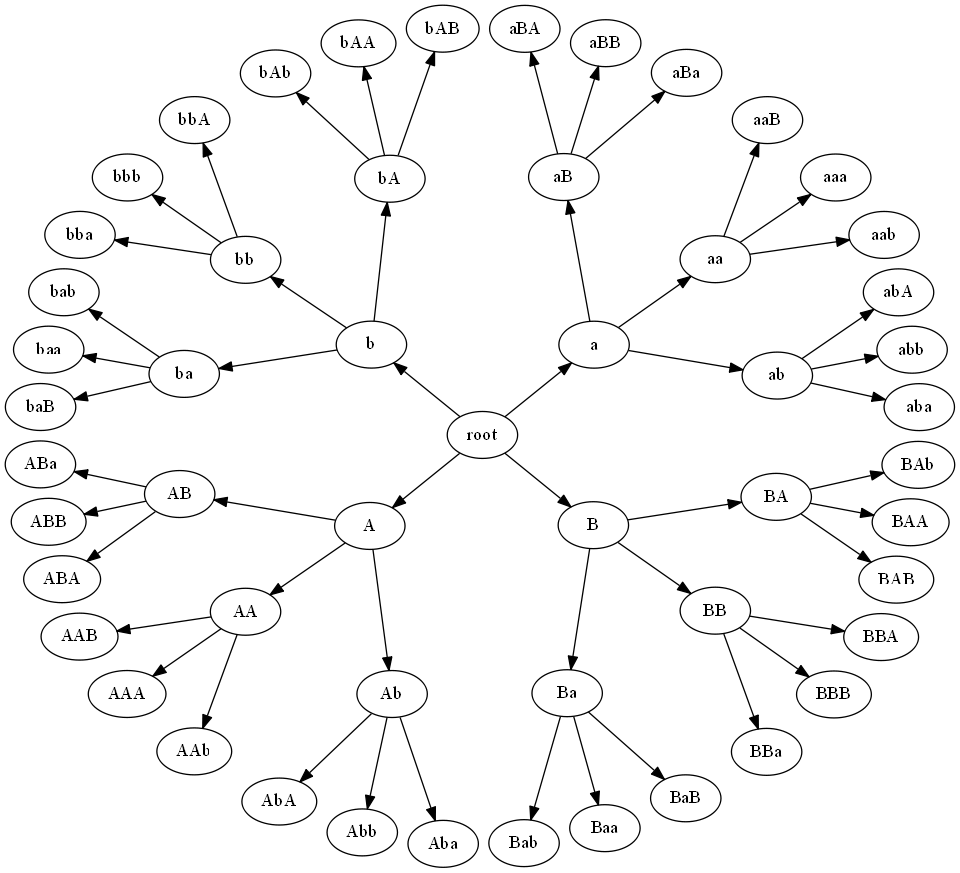
\includegraphics[height=1.35in, keepaspectratio]{img/cayleyGraph.png}
  \caption{\textit{Cayley Graph}}
  \label{fig:cayleyGraph}
  \hspace*{\fill}
 \end{minipage}
 \begin{minipage}[t]{0.333\hsize}
  \center
  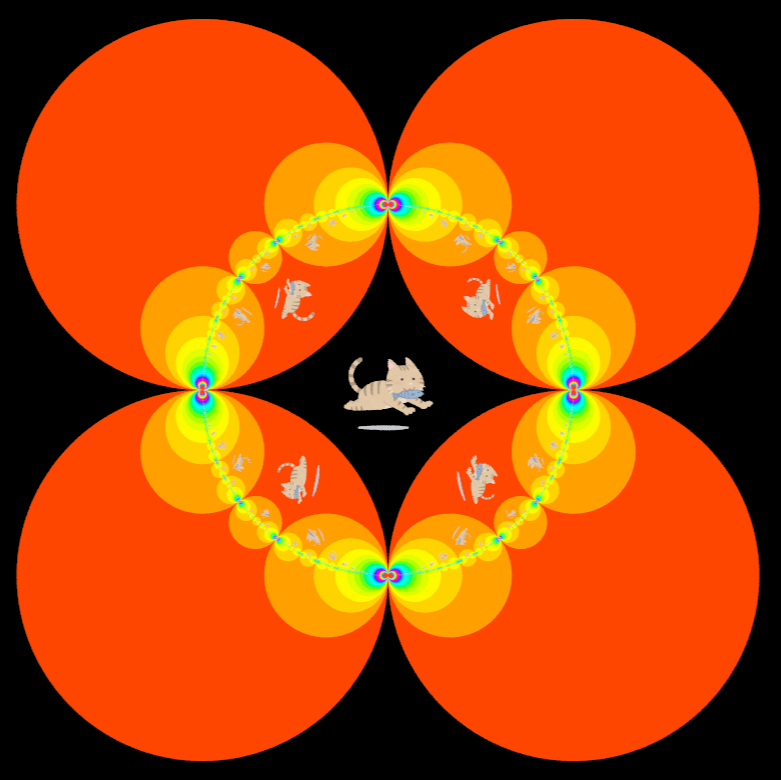
\includegraphics[height=1.35in, keepaspectratio]{img/preparation/basic/catOrbit.png}
  \caption{\textit{Orbit of the image}}
  \label{fig:orbitCat}
  \hspace*{\fill}
 \end{minipage}
 \begin{minipage}[t]{0.333\hsize}
  \center
  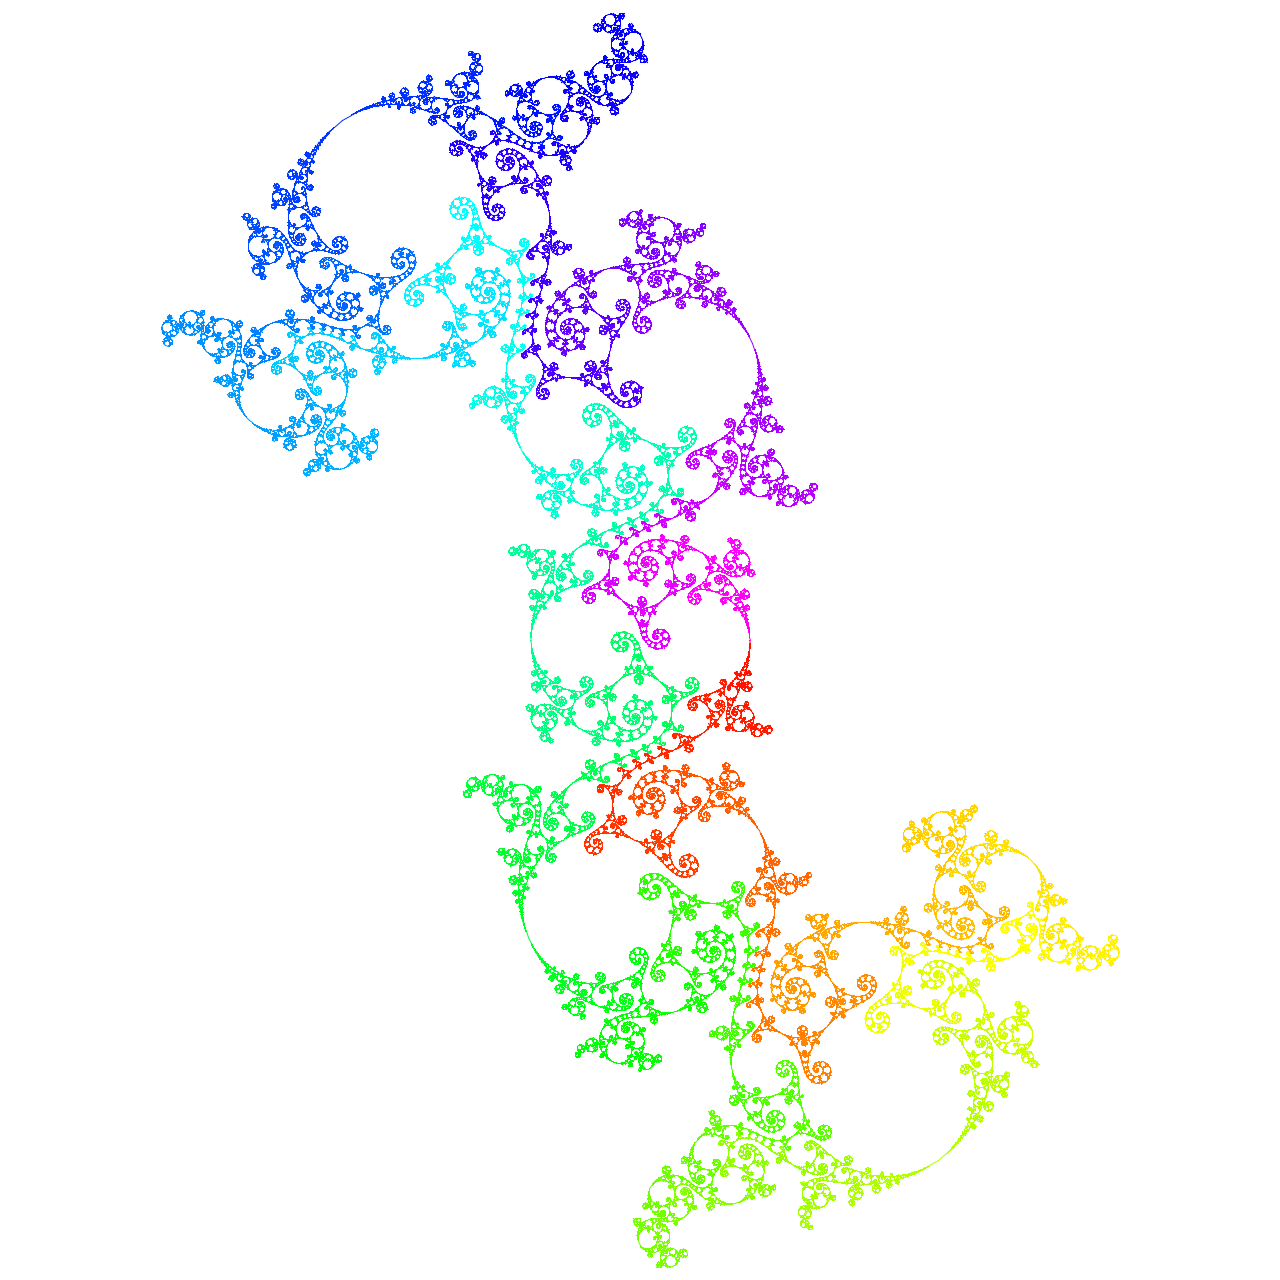
\includegraphics[height=1.35in, keepaspectratio]{img/preparation/limitSet/limit.png}
  \caption{\textit{Limit set of the Kleinian group}}
  \label{fig:limit}
  \hspace*{\fill}
 \end{minipage}
\end{figure}

\noindent In this sub-section, we introduce basic methods for visualizing Kleinian groups.
We consider \textit{cayley graph} of the Kleinian groups to enumerate elements
of the groups.
Figure \ref{fig:cayleyGraph} shows Cayley graph of the group generated
by two transformations.
The nodes of the graph show words.
They represent elements of the group.
Before we traverse the graph, we decide the maximum depth of traversing in advance.
According to the way of traversing the graph, 
there are two types of visualization of transformation groups.

Firstly, we can draw orbit of the group by traversing the cayley graph with
breadth first search. We can obtain words from the short ones.
See Figure \ref{fig:orbitCat}.%% TODO 画像をよいものに変更
The cat in the center is transformed by found words.
The circles and cats converges to the circle formed by disks.
We call the limiting disks the \textit{limit set} of the group.

Moreover, it is used to draw an tiling of the fundamental domain (tile.)
We can tile it by elements of the group.
If the group meet some conditions, we can tile them without gaps and
self intersections.%% TODO タイリングの画像をつける(Hyperbolic
                   %% Tessellationあたり)

Secondly, we can only draw the limit set of the group by traversing the
cayley graph with depth first search.
The limit set is located at the end of Cayley graph. Thus, we use fixed
point of the word.
After we traverse the graph, we obtain some long words.
We apply the words to the preselected fixed points of the group, and
we get limit set of the group as polygonal lines.
For more details, read Indra's Pearls.
Figure \ref{fig:limit} shows one of the limit set of the Kleinian group.

However, there are some faults in these methods.
For example, if we increase the number of generators,
It takes too much time to traverse the graph because of
combinatorial explosion.
Also, We have to traverse all of the graph
even though we don't need images outside of the screen.
This is the reason why we need other methods to visualize Kleinian
groups.

\subsection{Iterated Inversion System (IIS)}

\begin{figure}[htbp]
 \begin{minipage}[t]{0.16\hsize}
  \center
  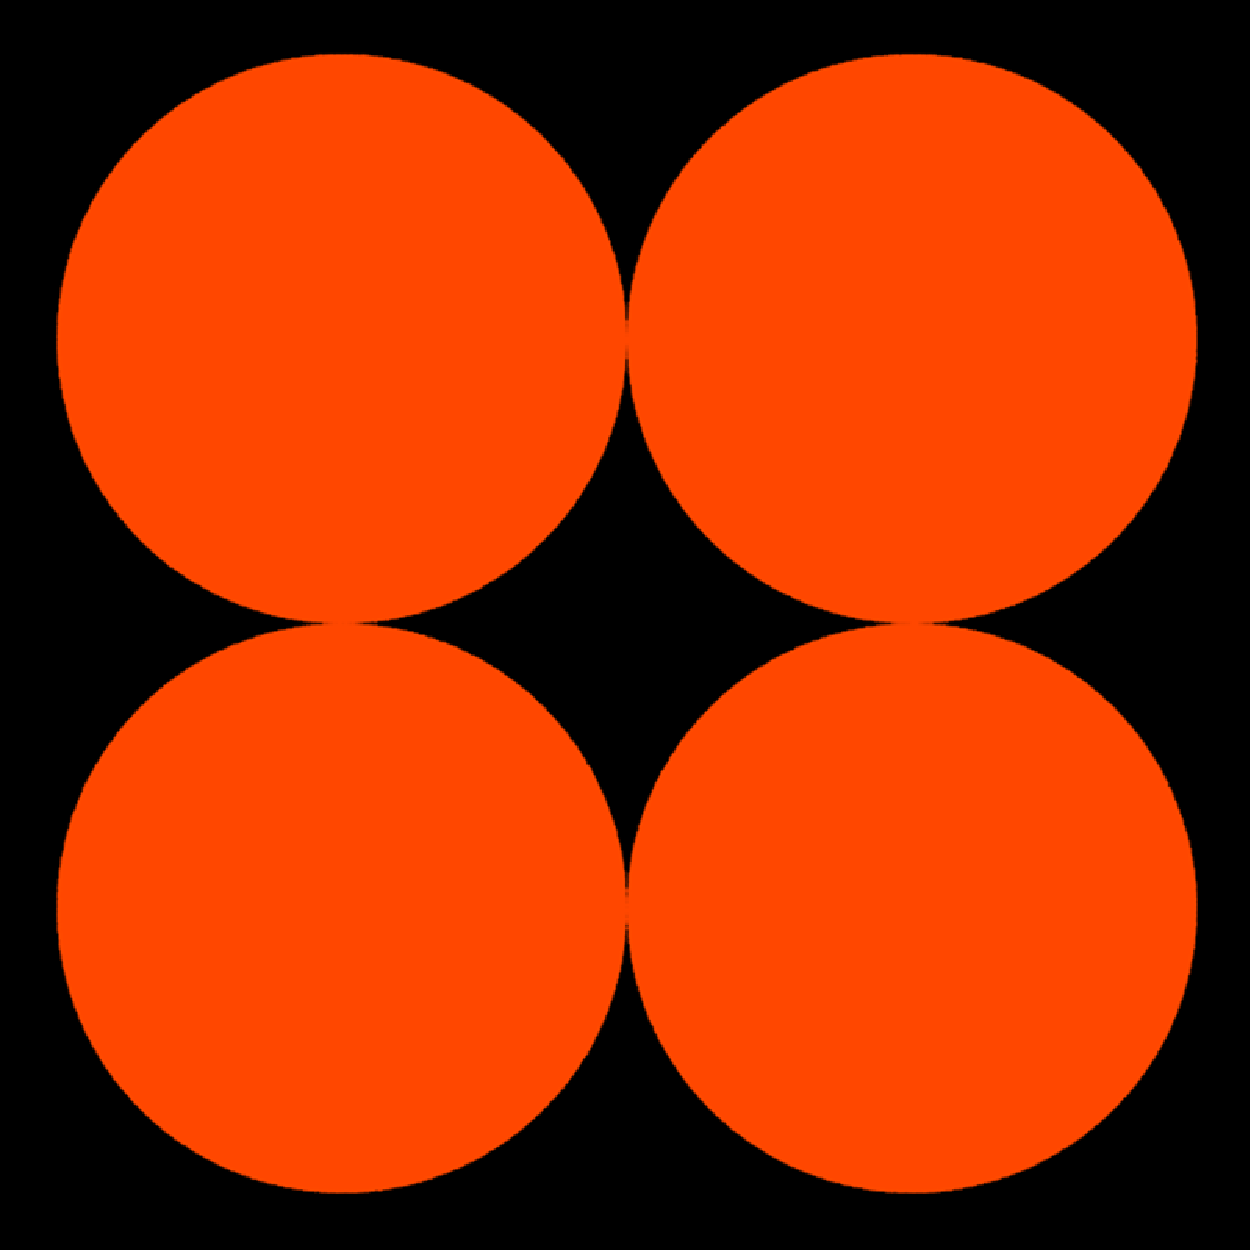
\includegraphics[width=1in, height=1in, keepaspectratio]{./img/preparation/orbit/level0c.pdf}
  \subcaption{}
  \label{fig:level0}
 \end{minipage}
 \begin{minipage}[t]{0.16\hsize}
  \center
  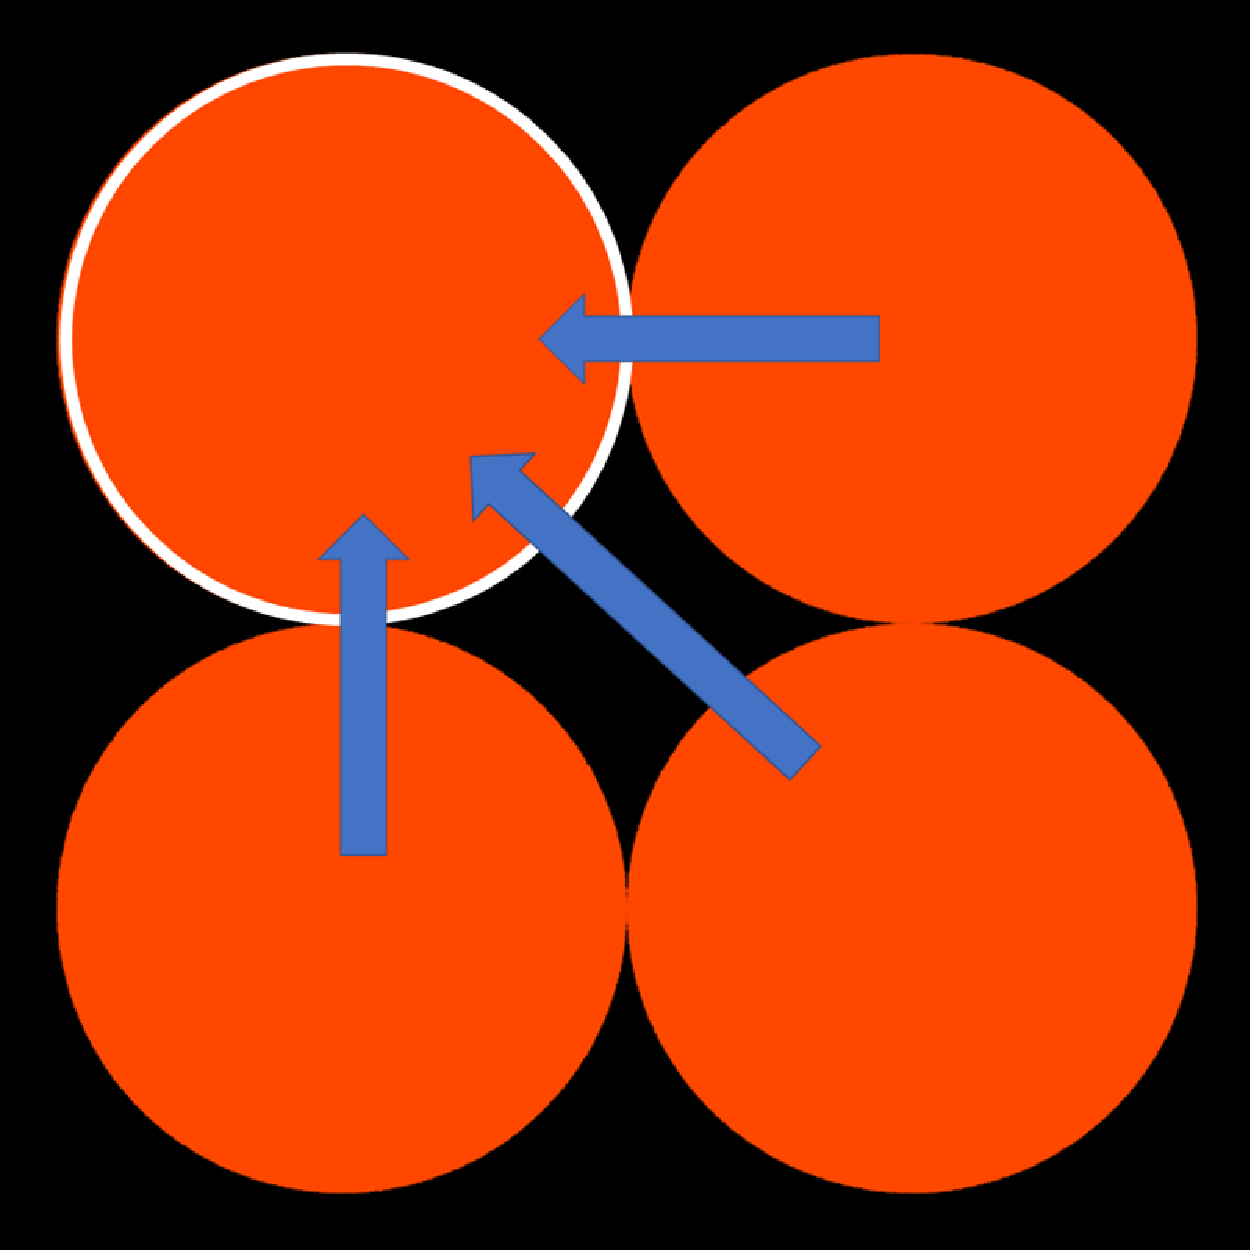
\includegraphics[width=1in, height=1in, keepaspectratio]{./img/preparation/orbit/level0invc.pdf}
  \subcaption{}
   \label{fig:level0inv}
 \end{minipage}
 \begin{minipage}[t]{0.16\hsize}
  \center
  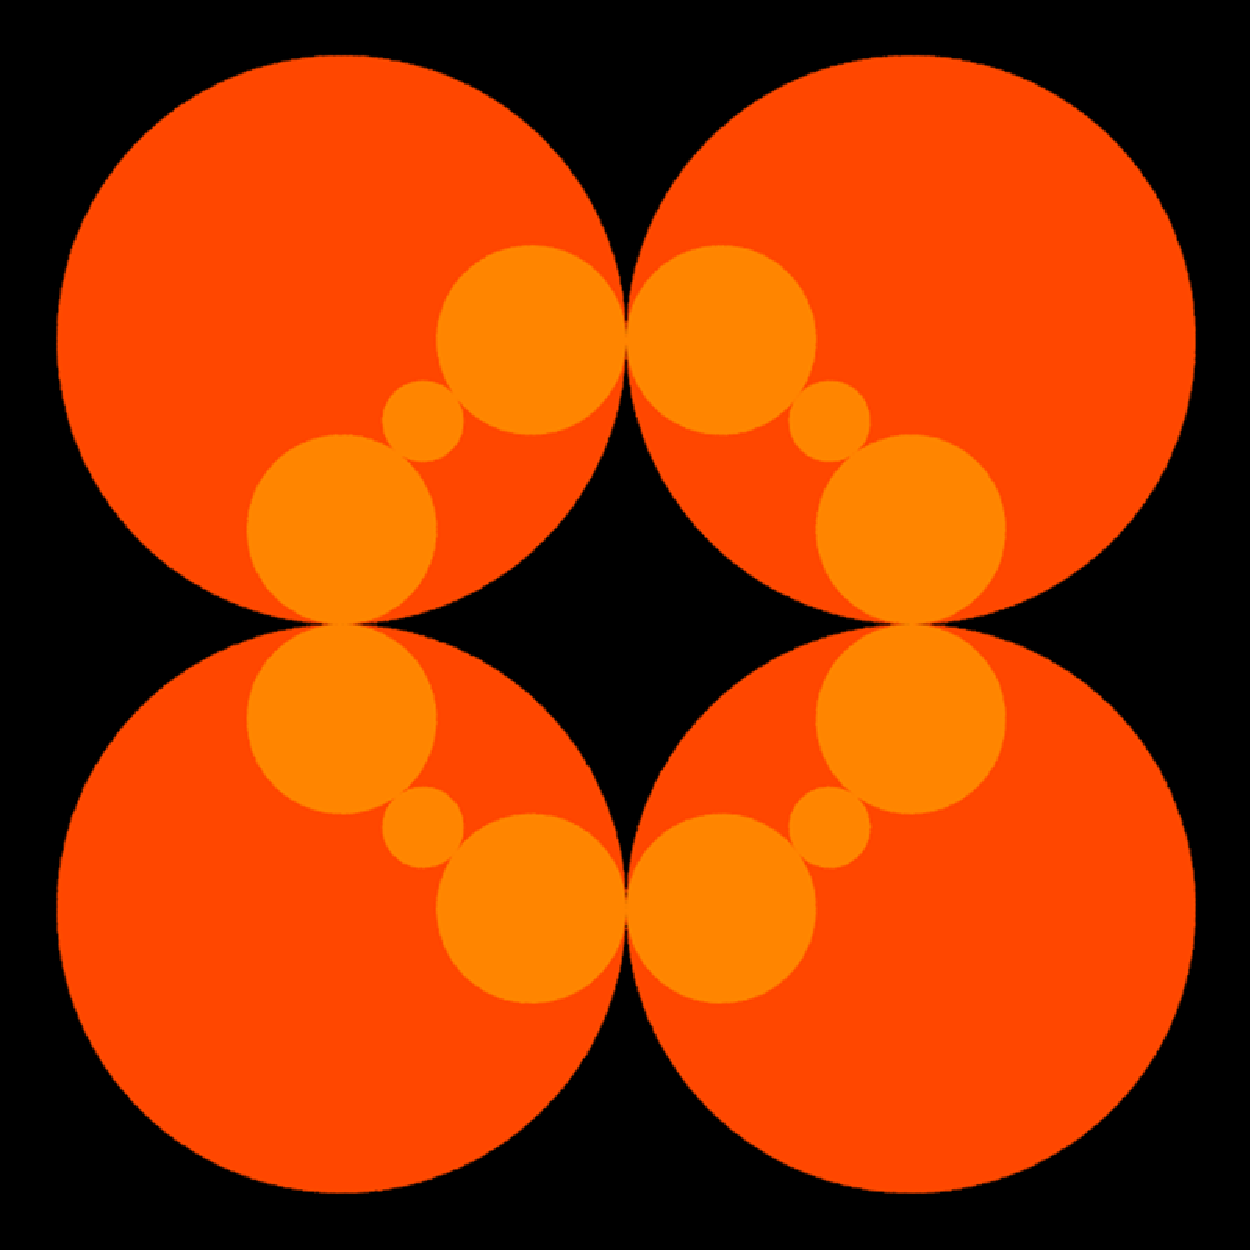
\includegraphics[width=1in, height=1in, keepaspectratio]{./img/preparation/orbit/level1c.pdf}
  \subcaption{}
   \label{fig:level1}
 \end{minipage}
 \begin{minipage}[t]{0.16\hsize}
  \center
  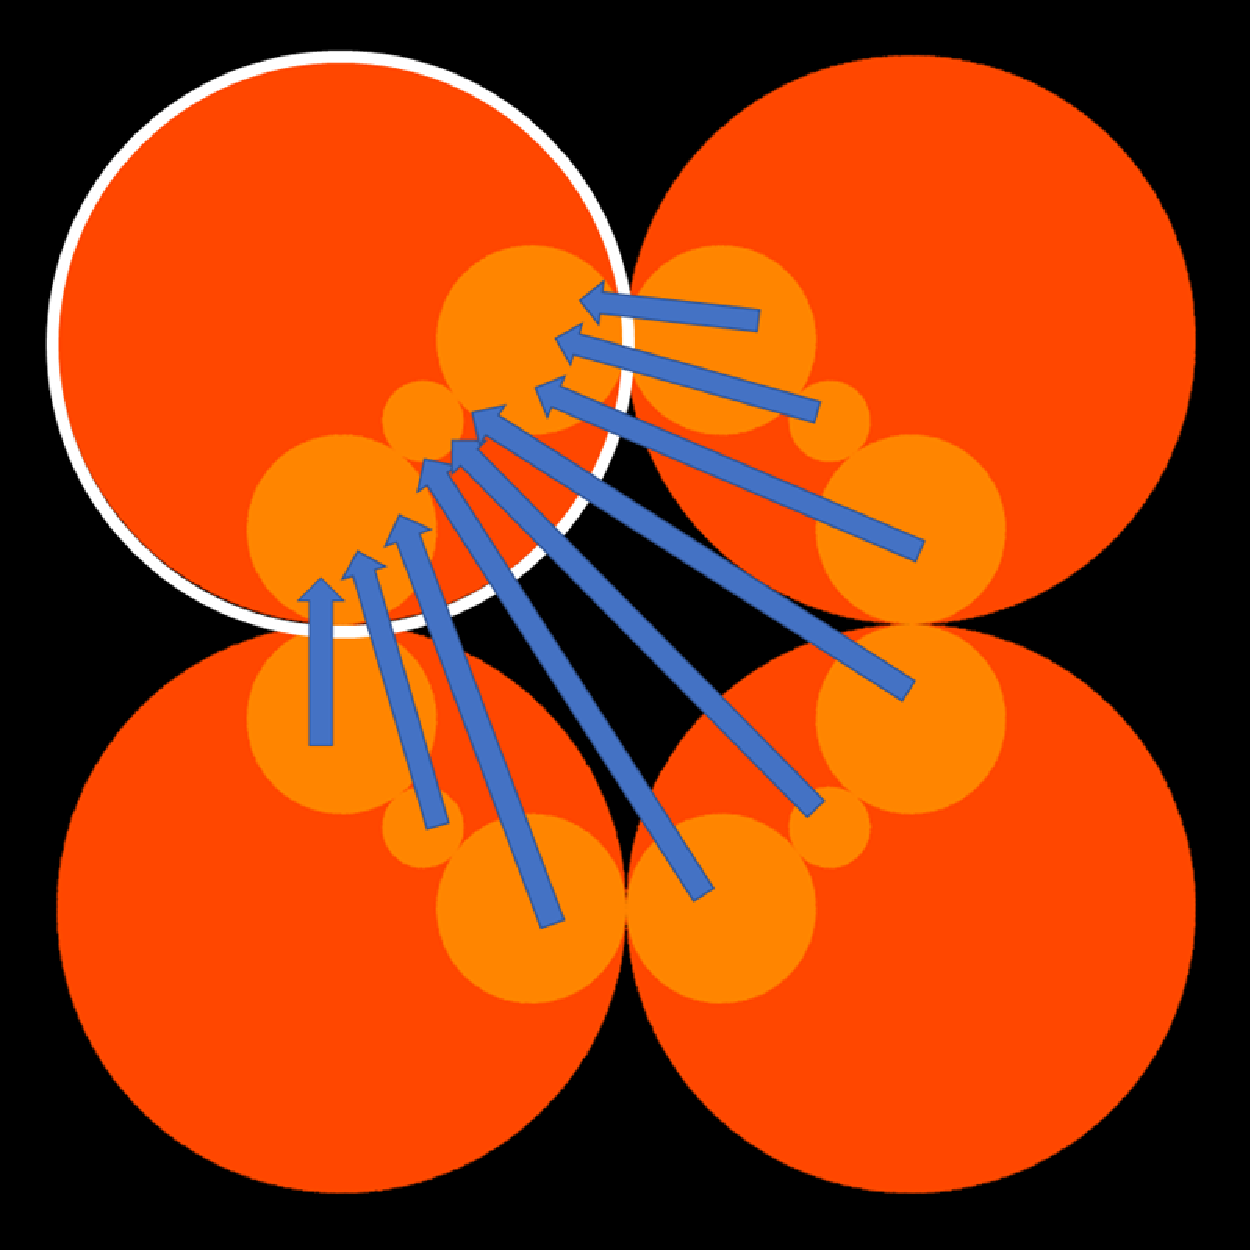
\includegraphics[width=1in, height=1in,
  keepaspectratio]{./img/preparation/orbit/level1invc.pdf}
  \subcaption{}
  \label{fig:level1inv}
 \end{minipage}
 \begin{minipage}[t]{0.16\hsize}
  \center
  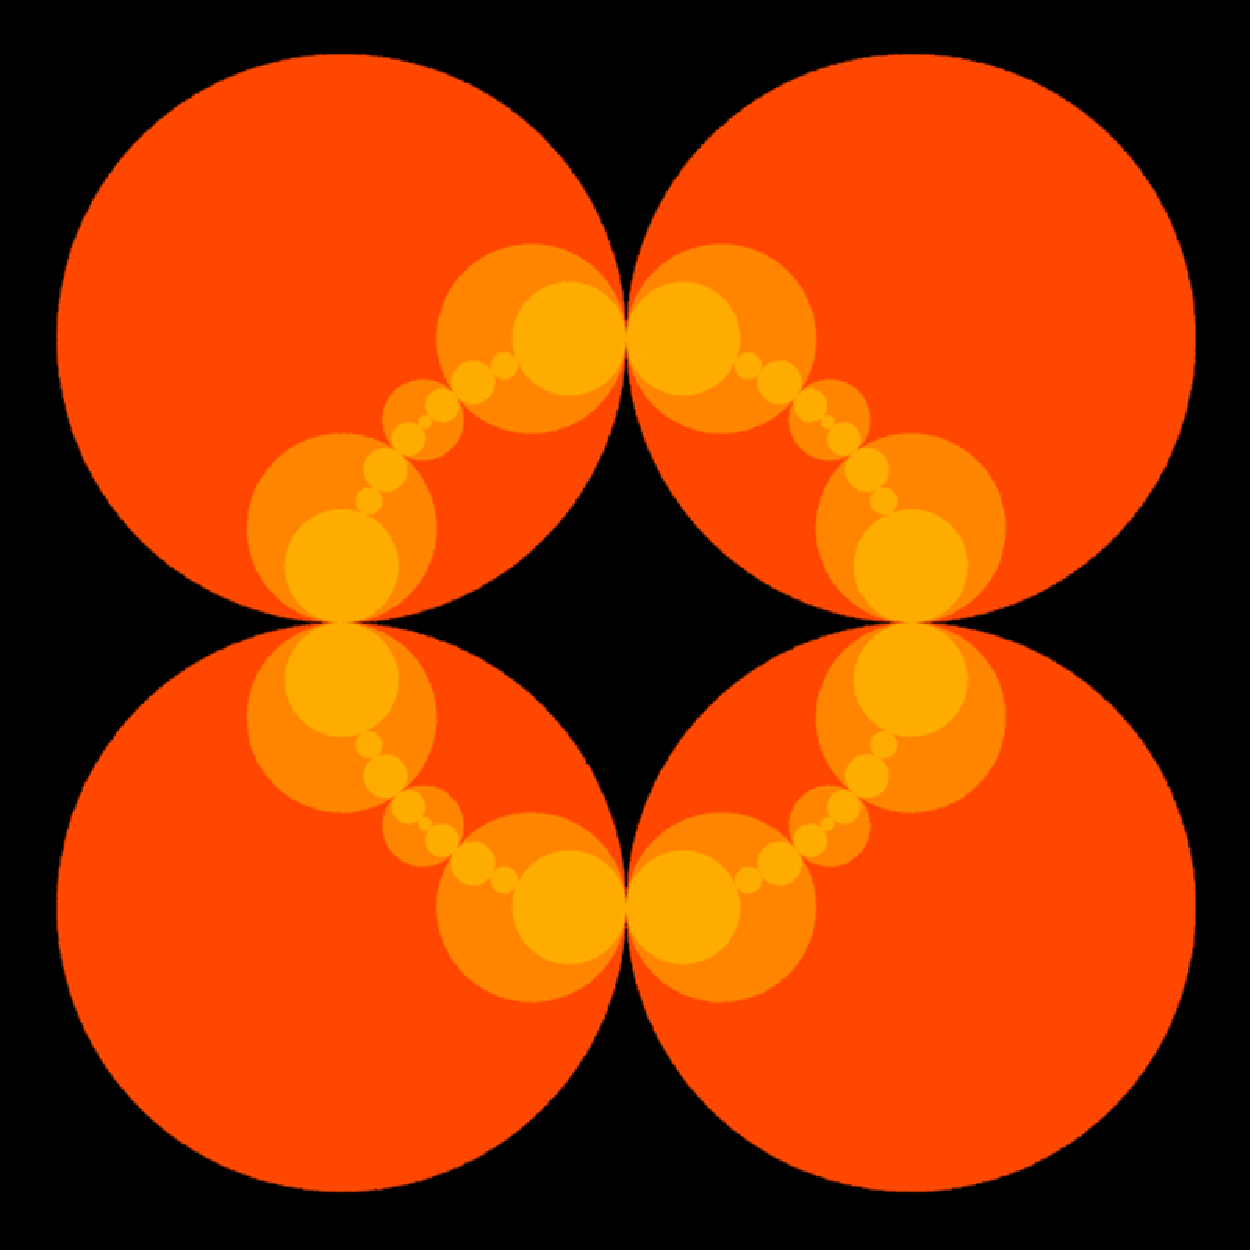
\includegraphics[width=1in, height=1in, keepaspectratio]{./img/preparation/orbit/level2c.pdf}
  \subcaption{}
  \label{fig:level2}
 \end{minipage}
 \begin{minipage}[t]{0.16\hsize}
  \center
  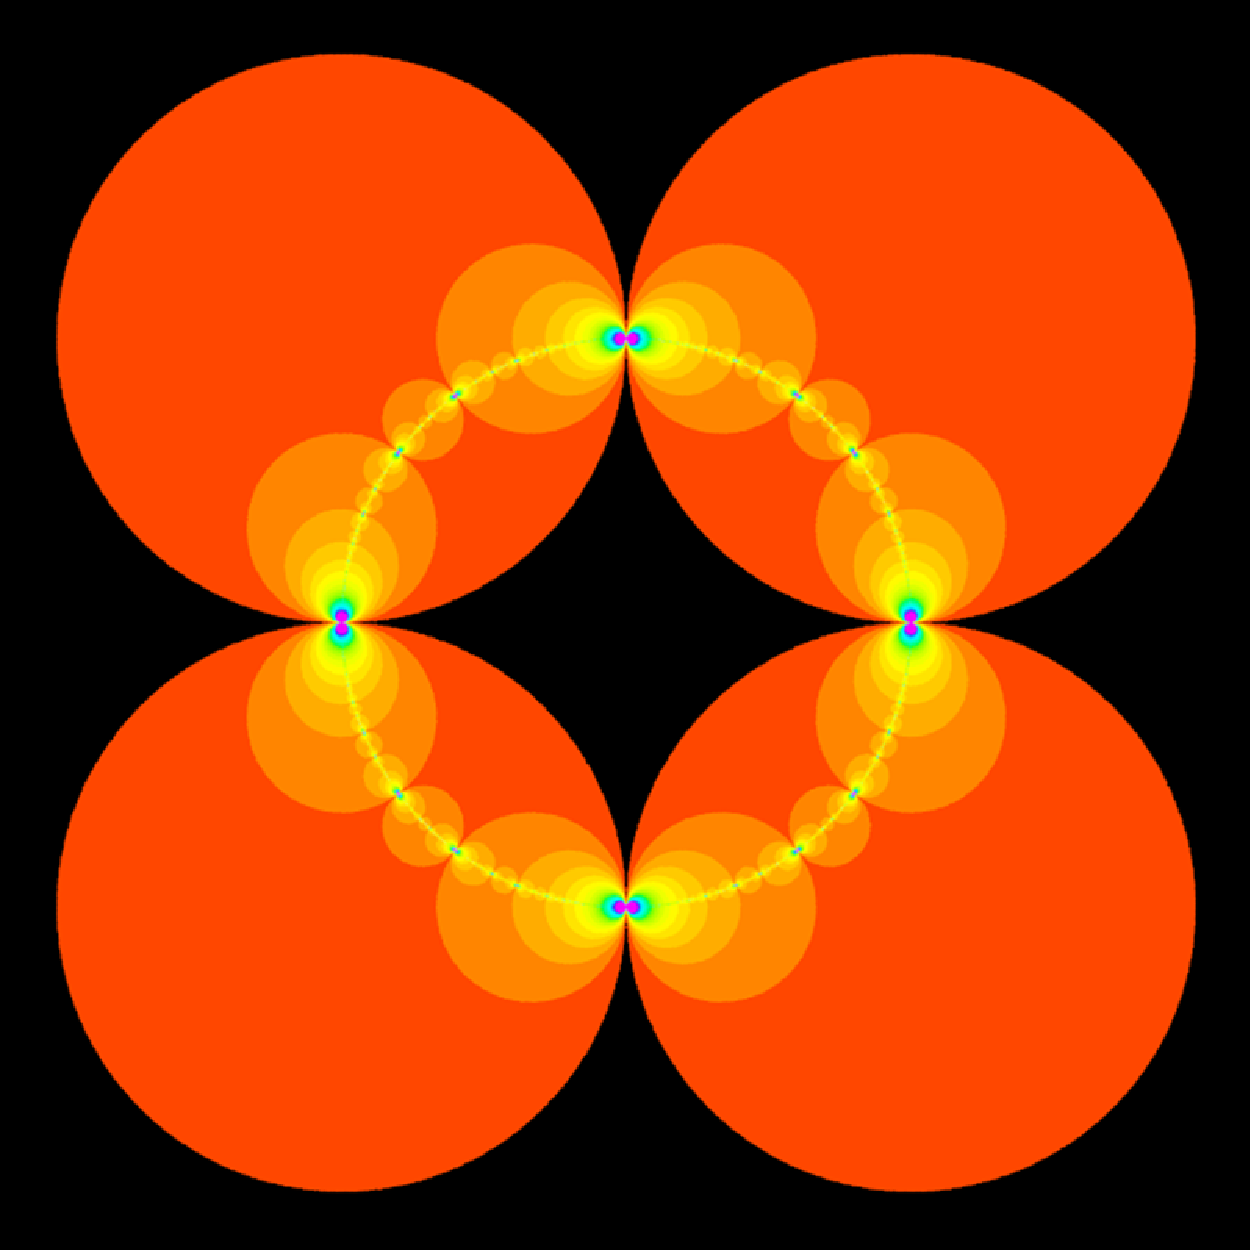
\includegraphics[width=1in, height=1in, keepaspectratio]{img/preparation/orbit/levelMaxc.pdf}
  \subcaption{}
  \label{fig:levelMax}
 \end{minipage}
 \caption{\textit{The process of rendering the orbit of Schottky disks}}
 \label{fig:schottkyProcess}
\end{figure}

\noindent To solve the problems we discussed in previous sub-section,
we focus circle inversions and invent an efficient algorithm to
visualize circle inversion fractals shown in Figure \ref{fig:schottkyProcess}\subref{fig:levelMax}.
The algorithm is called \textit{Iterated Inversion System (IIS.)}
It can visualize not only two dimensional circle inversion fractals but
also three dimensional sphere inversion fractals.

The fractal in Figure \ref{fig:schottkyProcess}\subref{fig:levelMax} shows the orbit of the first
four circles. %% TODO もうすこし説明を加える
It is also Kleinian group composed of four circle inversions.
Especially, it is also called a \textit{quasi-fuchsian group}.
The process of generation of circle inversion fractals is
as follows.

\begin{enumerate}
 \item We need some disjoint disks to obtain circle inversion fractals.
       For example, we assume there are four orange disks as shown in
       Figure \ref{fig:schottkyProcess}\subref{fig:level0}. We call orange disks \textit{initial
       disks} and their boundary \textit{initial circles}.
 \item First of all, we focus on the white circle in Figure
       \ref{fig:schottkyProcess}\subref{fig:level0inv}. The inversion in the white circle moves the
       other three disks into the interior of the white circle.
 \item After we apply each inversion in the initial circle to the outer disks,
       we obtain twelve small disks. They are shown in Figure \ref{fig:schottkyProcess}\subref{fig:level1}.
 \item Next, we invert the twelve small disks in the initial circles.
       The inversion in the white circle moves the outer nine small disks
       into the interior of the white circle as shown in Figure \ref{fig:schottkyProcess}\subref{fig:level1inv}.
       Each inversion in the Schottky circle generates smaller disks, and we
       obtain Figure \ref{fig:schottkyProcess}\subref{fig:level2}.
 \item We continue iterating these process, that is, we continue
       applying each inversion in the initial circle to resulting
       smaller disks.
       Finally, we get Figure \ref{fig:schottkyProcess}\subref{fig:levelMax}.
\end{enumerate}

\subsubsection{Two Dimensional IIS}

\begin{figure}[htbp]
  \center
  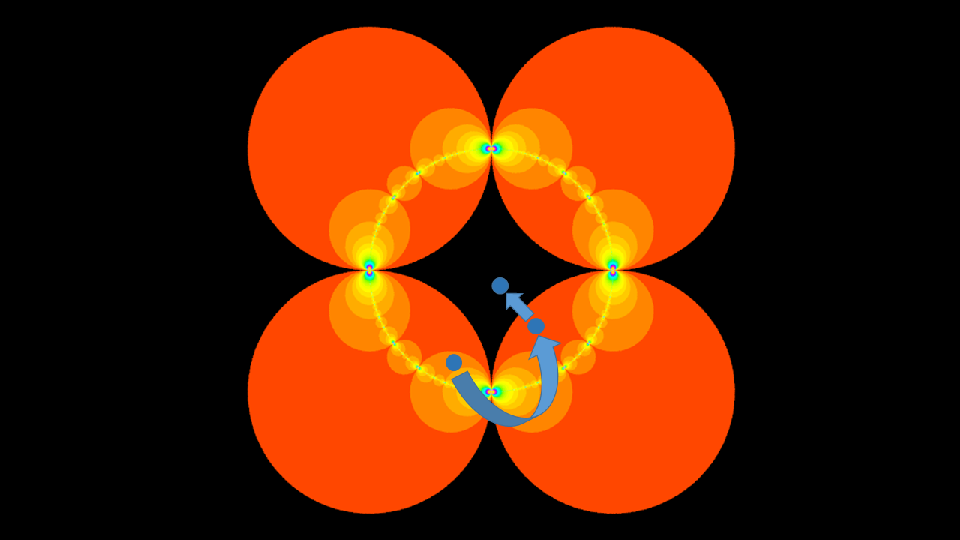
\includegraphics[height=1.35in, keepaspectratio]{img/preparation/orbIIS.png}
  \caption{\textit{Orbit of blue point by IIS}}
  \label{fig:iisOrbit}
 \hspace*{\fill}
\end{figure}

 \begin{algorithm}
  \caption{Iterated Inversion System (IIS)}
  \label{arg:iis2d}
  \begin{algorithmic}
   \REQUIRE count $= 0$ and coordinates $=$ position determined by
   pixel
   \FOR{$i=0$ to MAX\_INVERSION}
   \STATE inOutside $\leftarrow$ \TRUE
   \FOR{ each Map $G$ in circles }
   \IF{$G$ is available to coordinates}
   \STATE coordinates $\leftarrow$ $G(\text{coordinates})$
   \STATE INCREMENT count
   \STATE inOutside $\leftarrow$ \FALSE
   \ENDIF
   \ENDFOR
   \IF {inOutside}
   \STATE BREAK for
   \ENDIF
   \ENDFOR
   \STATE RETURN count
  \end{algorithmic}
 \end{algorithm}

\noindent IIS computes the depth of the circles point by point.
Thus, we can perform parallel processing and render the images efficiently.
The images in this paper are rendered using \textit{OpenGL Shading
Language (GLSL)}.

IIS is applied to each point on the plane and computes nesting depth of
the disk which contains the point.
The process of the algorithm is as follows.
First of all, if the point is contained in initial disks, we invert the
point in the boundary circle of the disk.
We continue applying inversions until the transformed point is in the
outside of the initial disks.
Figure \ref{fig:iisOrbit} shows orbit of the blue point transformed by
iterations of inversions.

Furthermore, a point actually at the limit set never reaches the
outside. So, we have to determine the maximum number of iterations in
advance to prevent the algorithm from running indefinitely.
The points except for the limit set are guaranteed that they
are transformed to outside because inversions are involution.

Pseudo-code of IIS is shown in Algorithm \ref{arg:iis2d}.
Later, we will introduce generators other than simple inversions.
Thus, we consider a map $G$ such that $G$ is an identity for a point in the
\textit{fundamental domain} and that $G$ is a composition of inversions for other
points.
The fundamental domain is the terminal area of transformations. 
In the above case, the black area where outside of all circles.

\subsubsection{Three Dimensional Extension}

\begin{figure}[htbp]
 \begin{minipage}[t]{0.5\hsize}
  \center
  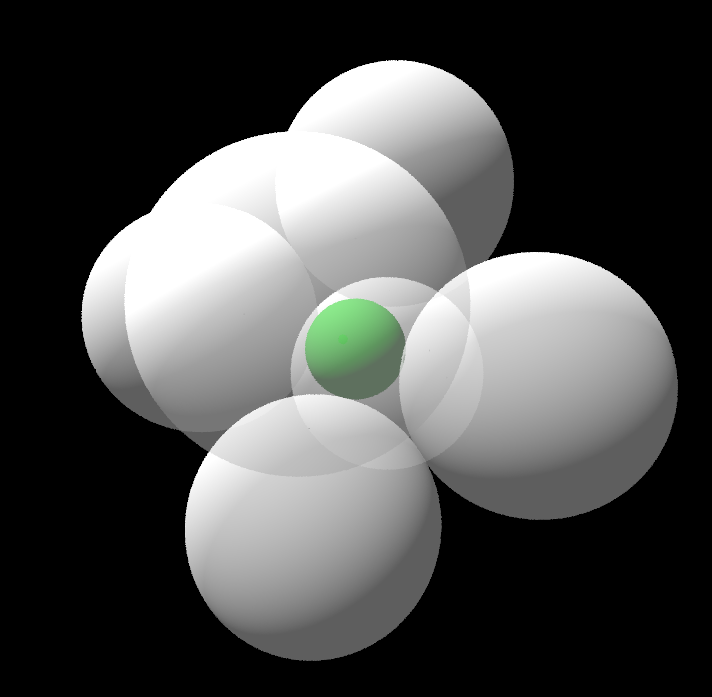
\includegraphics[height=1.35in, keepaspectratio]{img/preparation/3dExtension/3dKissingGenerator.png}
  \subcaption{\textit{Generator}}
  \label{fig:simpleGen}
  \hspace*{\fill}
 \end{minipage}
 \begin{minipage}[t]{0.5\hsize}
  \center
  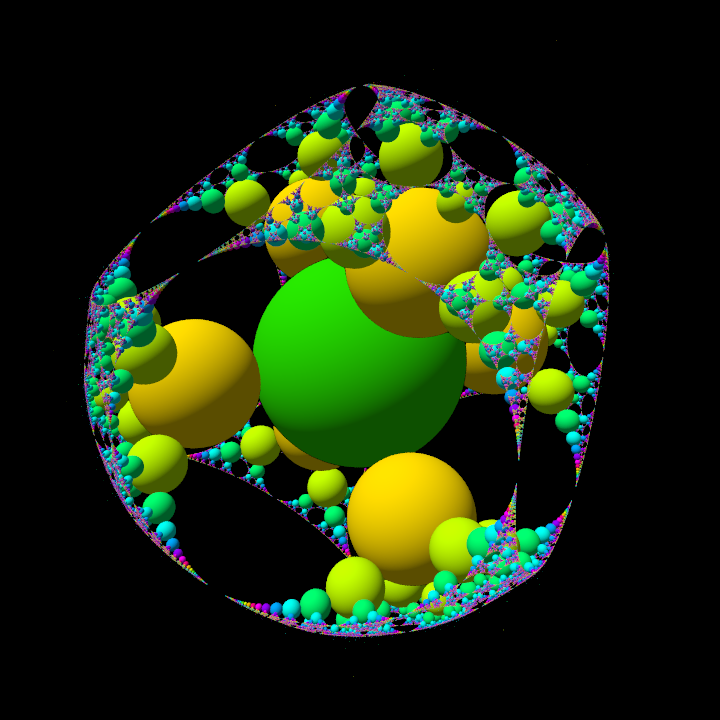
\includegraphics[height=1.35in, keepaspectratio]{img/preparation/3dExtension/3dOrbit.png}
  \subcaption{\textit{The orbit of spheres}}
  \label{fig:simpleOrb}
  \hspace*{\fill}
 \end{minipage}
 \caption{\textit{The orbit of the sphere inversion fractal}}
 \label{fig:simpleGenOrb}
\end{figure}

In the similar manner to two dimensional algorithm,
we extend the IIS to visualize three-dimensional kleinian groups.
We extend circle inversion to sphere inversion easily, and we
compute the nesting depth of the sphere voxel by voxel.

We use \textit{ray tracing} to visualize three dimensional objects.
Ray tracing computes intersection between ray and objects algebraically.
There are two ways to render nesting spheres. First one is to draw
nesting spheres as transparent spheres.
Second one is \textit{volume rendering}.
However, these are difficult to render them efficiently, and
visualized images are not interesting.

Therefore we render the orbit of sphere in a similar way to the two
dimensional circle inversion fractals.
See Figure \ref{fig:simpleGenOrb}\subref{fig:simpleGen}. It shows
white six inversion spheres and green seed sphere.
Figure \ref{fig:simpleGenOrb}\subref{fig:simpleOrb} shows the orbit of
green sphere transformed by inversions in white spheres.

We use \textit{Sphere Tracing} \cite{hart1996sphere} to render three dimensional
fractals and orbit of the seed sphere.
Sphere Tracing is one of the algorithm to render implicit surfaces using
ray tracing.
In the following paragraphs, we introduce ray tracing and
 sphere tracing.

In the first place, we work a ray as something like a vector.
We set the origin of the ray to the position of the camera
and direction of the ray to the direction to each pixel on the screen
from the camera. Each pixel is colored according to the
first object the ray hits. 

In regular ray tracing, we calculate the intersections algebraically, but
we can not compute intersection to fractal objects.
On the other hand, in sphere tracing, we march the ``tip'' of the ray
along the direction of the ray step by step. 
To check how far the tip of the ray is from the objects, we need a
\textit{distance function}.
Distance function is a function which returns minimum distance between
given point and objects.
For example, a distance function of a sphere is as follows.
Let $P$ be a tip of a ray, let $C$ and $R$ be center and
radius of the sphere.
Distance function $f(x)$ is $f(x) = distance(P, C) - R$ where $x$ is tip
of the ray.
If there are many spheres, we use minimum distance to the sphere.

However, in regard to fractal rendering, it is difficult to
get an actual distance to its shape. So, we use lower estimated distance
as a return value of the distance function. The technique to approximate
distance is called \textit{distance estimation}.
For more details about fractal rendering and distance estimation, see also the blog
post\footnote{Mikael H Christensen, Distance Estimated 3D Fractals (Part I):\\ \quad\quad
\url{http://blog.hvidtfeldts.net/index.php/2011/06/distance-estimated-3d-fractals-part-i/}}
by Christensen. 

\begin{figure}[htbp]
 \begin{minipage}[t]{0.5\hsize}
  \center
  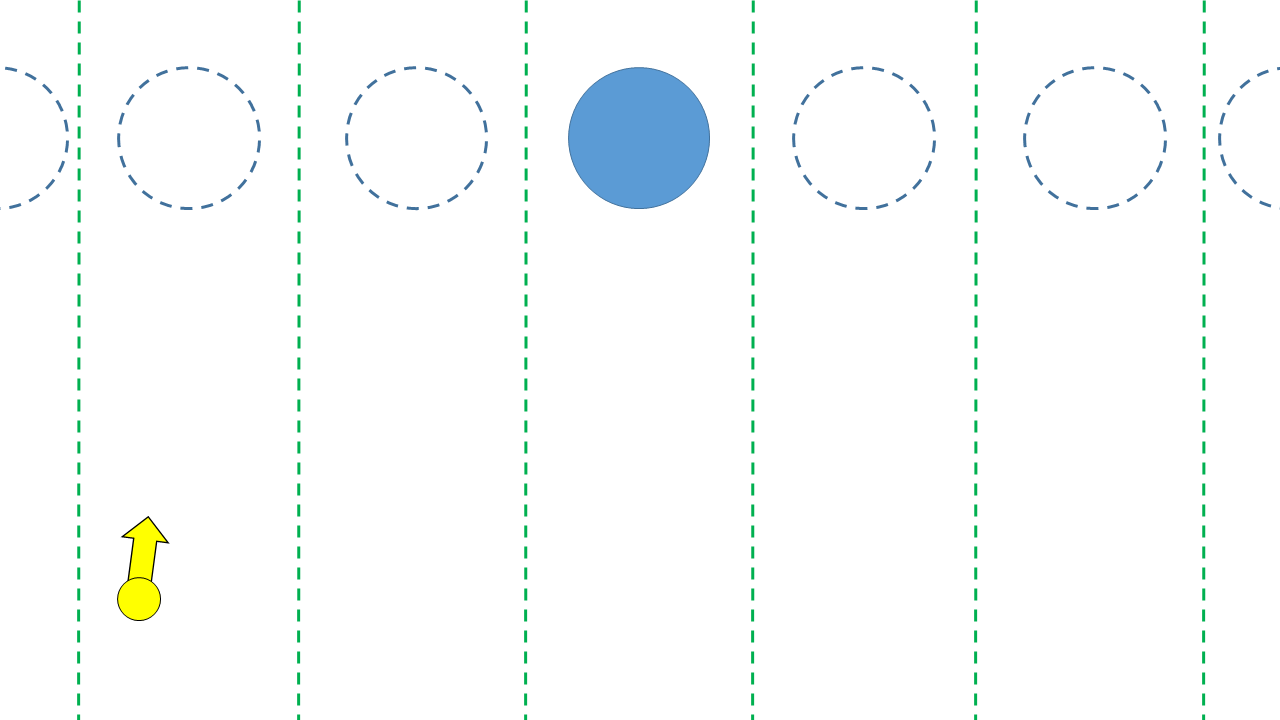
\includegraphics[height=1.35in, keepaspectratio]{img/preparation/iis3d/modulo1.png}
  \caption{\textit{modulo1}}
  \label{fig:modulo1}
  \hspace*{\fill}
 \end{minipage}
 \begin{minipage}[t]{0.5\hsize}
  \center
  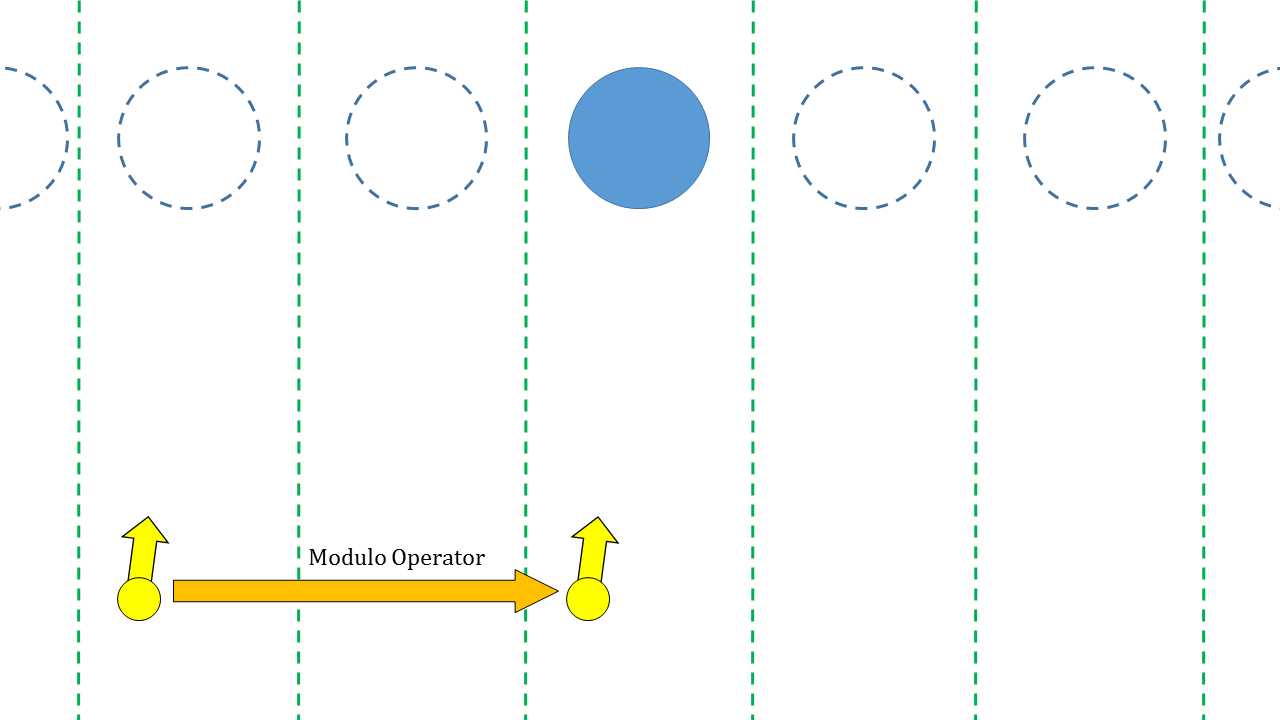
\includegraphics[height=1.35in, keepaspectratio]{img/preparation/iis3d/modulo2.png}
  \caption{\textit{Fold space by modulo operator}}
  \label{fig:modulo2}
  \hspace*{\fill}
 \end{minipage}
\end{figure}

Before we introduce distance estimation, we show
well known technique to render many objects in sphere tracing.
Instead of preparing distance functions for many objects, we can use modulo operator
to get distance to the lined up objects.

See Figure \ref{fig:modulo1}. We assume there are blue disk, yellow  ray and dotted
circle and lines.
Now, we want to draw all of the dotted circles.
So, we want to minimum distance between the ray and dotted circles.
However we only know the position of the tip of the ray and the blue disk.
We assume the nearest circle to the ray is in same dotted region, and
we fold up the regions using modulo operator.
We can measure distance to blue disk as in Figure \ref{fig:modulo2}.
Finally, we can draw line upped disks.

\begin{figure}[htbp]
 \begin{minipage}[t]{0.5\hsize}
  \center
  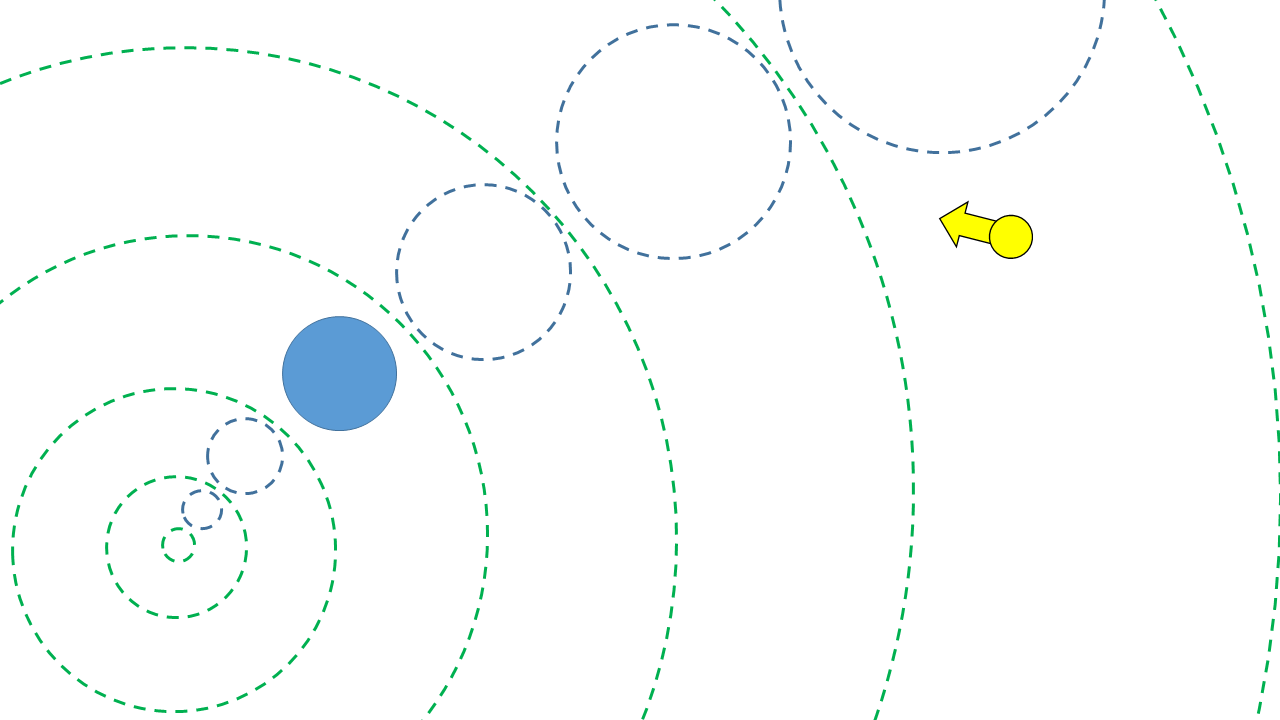
\includegraphics[height=1.35in, keepaspectratio]{img/preparation/iis3d/scaleIIS.png}
  \caption{\textit{scaling1}}
  \label{fig:iisScale1}
  \hspace*{\fill}
 \end{minipage}
 \begin{minipage}[t]{0.5\hsize}
  \center
  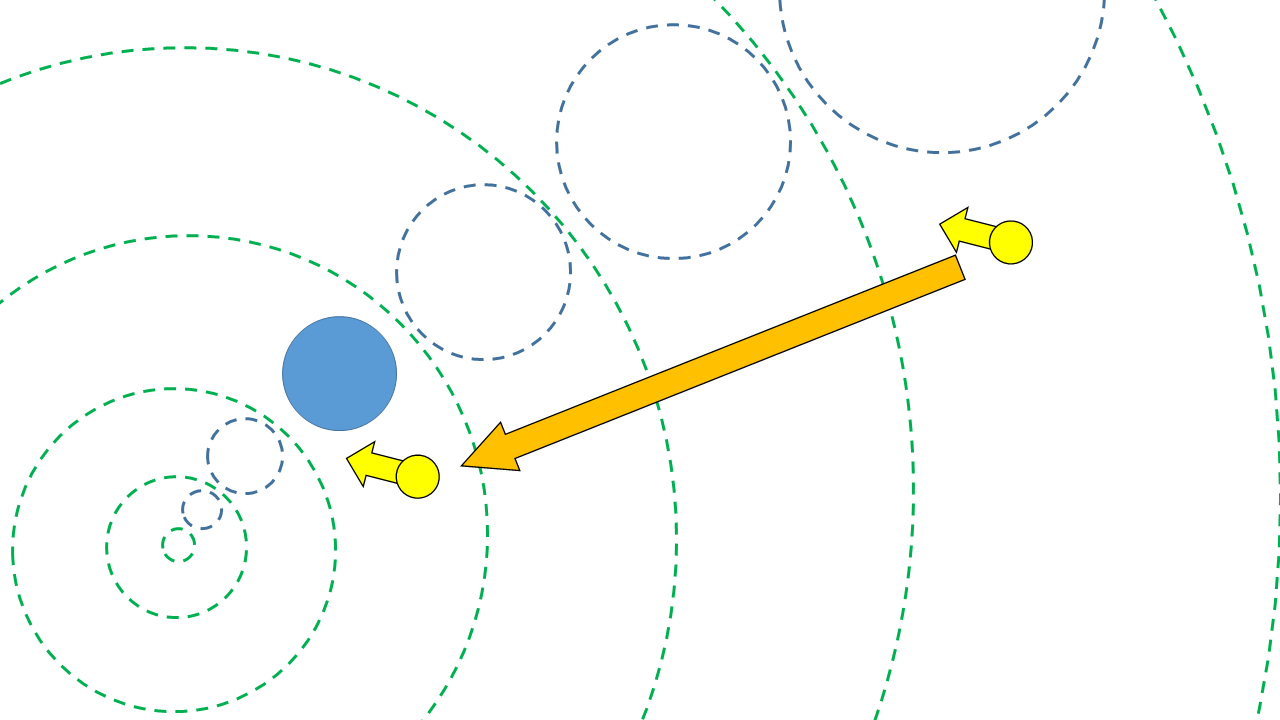
\includegraphics[height=1.35in, keepaspectratio]{img/preparation/iis3d/scaleIIS2.png}
  \caption{\textit{scaling2}}
  \label{fig:iisScale2}
  \hspace*{\fill}
 \end{minipage}
\end{figure}

Next, we consider scaling example. See Figure \ref{fig:iisScale1}.
There is a yellow ray and a blue disk, and orbit of scaling as
dotted blue circles.
The green dotted lines show scaling regions.
We want to minimum distance to dotted blue circles.
We assume that the nearest sphere to the tip of the ray is at
same regions. 
However, we only know the coordinates of the original blue
disk and tip of the ray.
Thus, we scale the tip of the ray to the same region to the blue disk
but, the distance between scaled ray and disk is also scaled.
So, we correct the scale dividing computed distance by 
Jacobian (sometimes referred to as the Jacobian determinant) of scaling.
See Figure \ref{fig:iisScale2}.
If the scaling of the circle is $f(x) = 2x$, we divide the scale by
eight because the ray is moved three green scaling region.

\begin{figure}[htbp]
 \begin{minipage}[t]{0.5\hsize}
  \center
  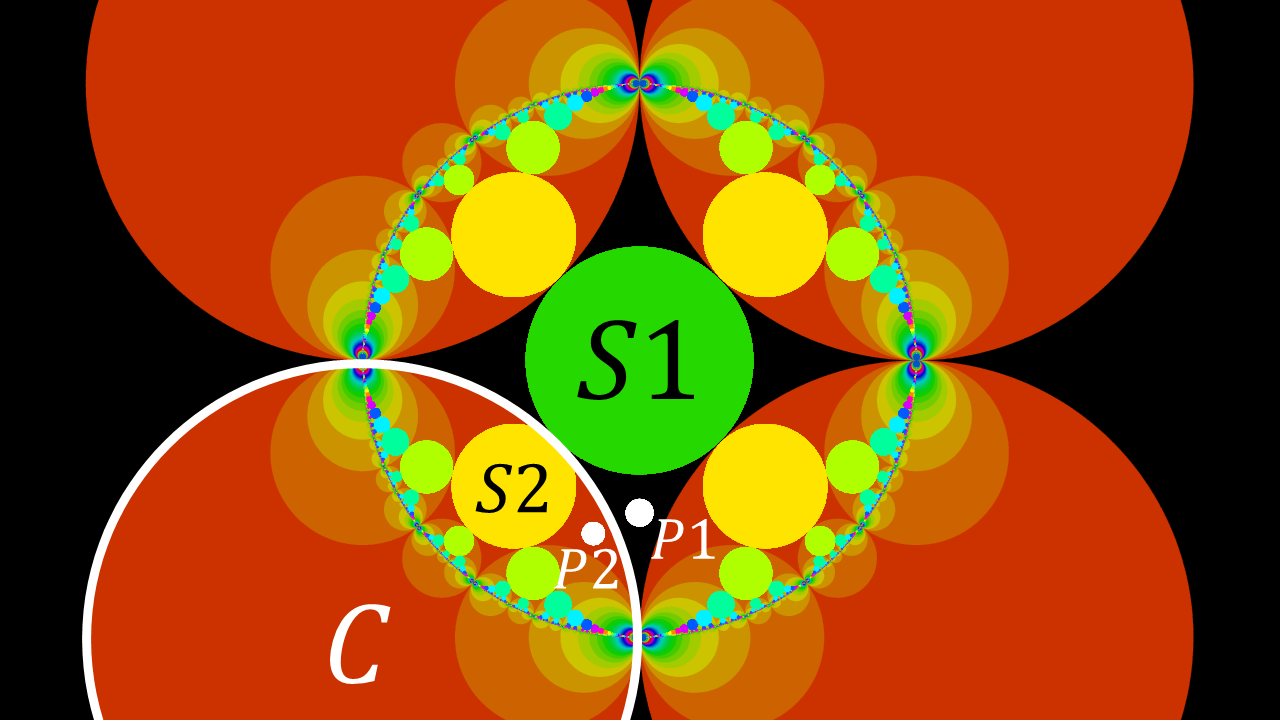
\includegraphics[height=1.35in, keepaspectratio]{img/preparation/slice.png}
  \caption{\textit{XY-slice image of Figure \ref{fig:simpleGenOrb}\subref{fig:simpleOrb}}}
  \label{fig:slice2d}
  \hspace*{\fill}
 \end{minipage}
 \begin{minipage}[t]{0.5\hsize}
  \center
  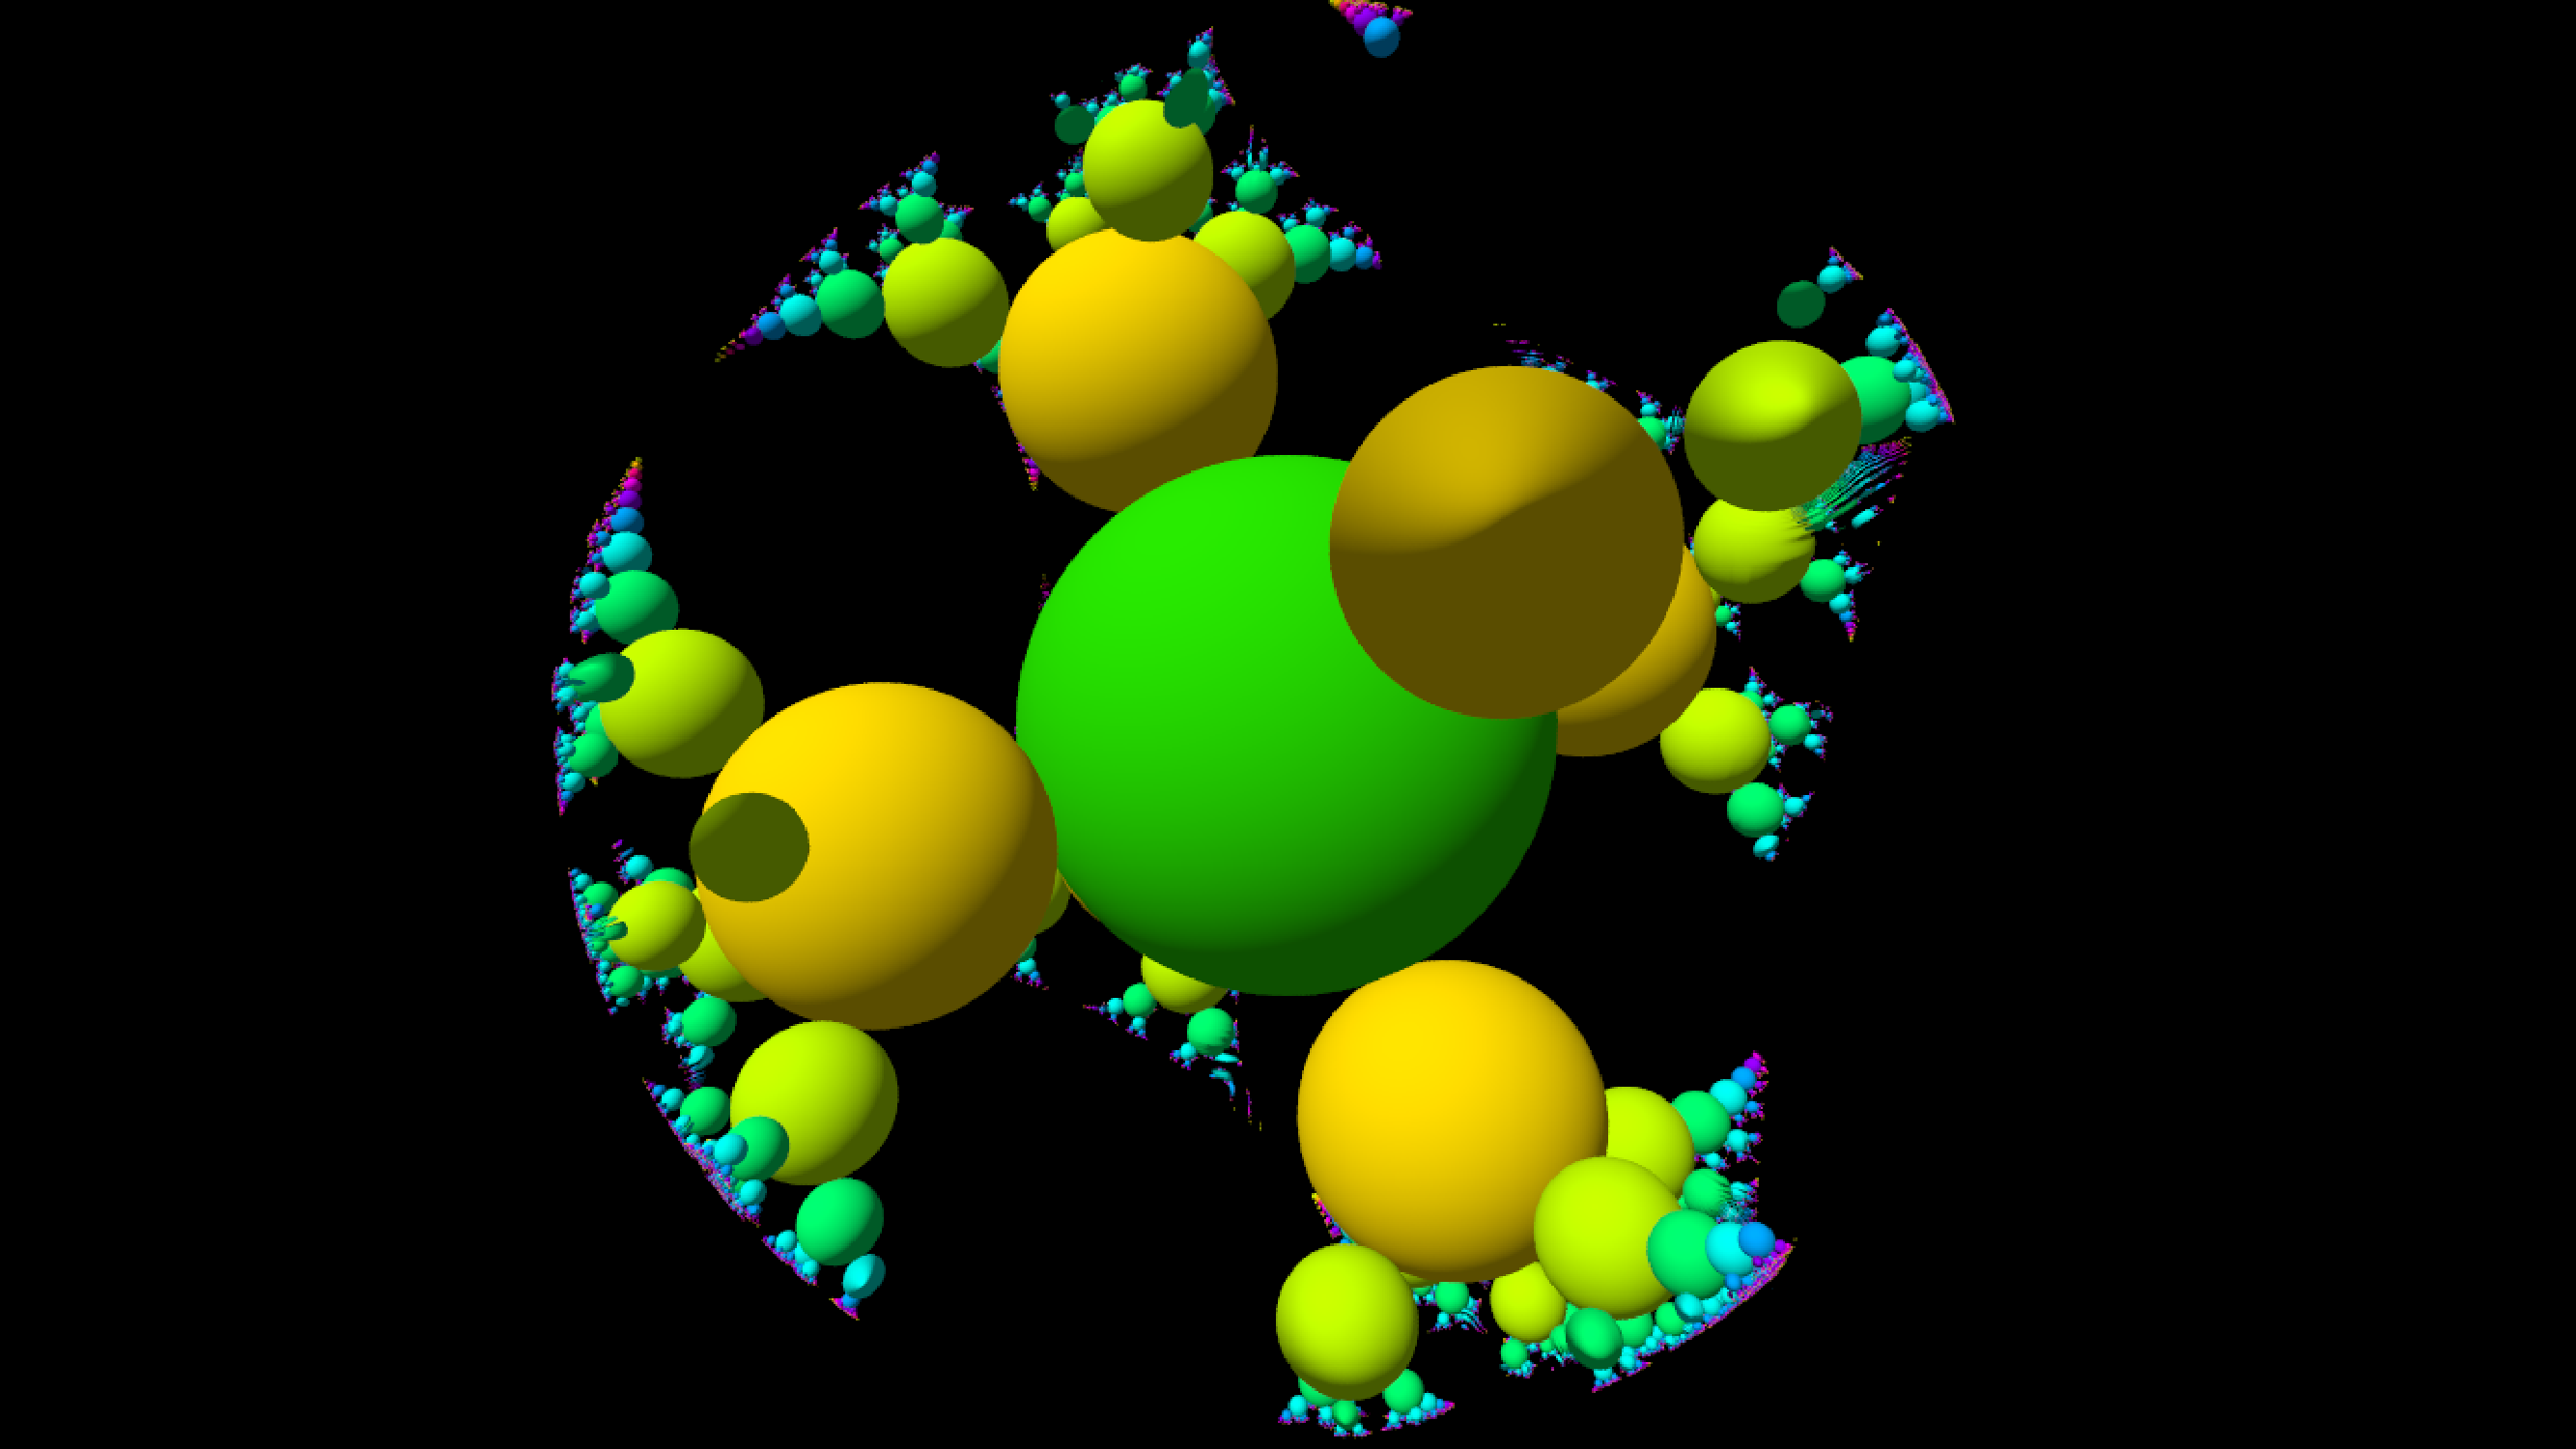
\includegraphics[height=1.35in, keepaspectratio]{img/preparation/artifact.pdf}
  \caption{\textit{artifact}}
  \label{fig:3dartifact}
  \hspace*{\fill}
 \end{minipage}
\end{figure}

In the similar manner to scaling, we can render sphere inversion
fractals.
For the sake of simplicity, we consider a slice image of Figure
\ref{fig:simpleGenOrb}.
See Figure \ref{fig:slice2d}. This image shows the XY-slice of the orbit
of spheres.
Orange disks in background  are slices of the orbit of initial inversion spheres.
Slices of the orbit of the base sphere are colored in
the same color as the orbit shown in Figure \ref{fig:simpleGenOrb}\subref{fig:simpleOrb}.
$C$ is the white circle, the boundary of the initial inversion sphere.
$S1$ is the base sphere and the inversion of $S2$ in the circle $C$. 
The white point $P1$ is the inversion of $P2$ in the circle $C$.

Now we assume that the tip of the ray is at $P2$.
Let's calculate the minimum distance between
$P2$ and the orbit of base spheres.
The nearest sphere to $P2$ is $S2$.
So, we have to calculate the distance between $P2$ and $S2$.
We call the distance $d$.
However, we do not know the center and radius of $S2$.
So, we calculate $d$ from a distance between $S1$ and $P1$.
Inversions in spheres and M\"obius transformations do not preserve
Euclidean distance.
Thus we use the Jacobian to estimate the distance.
We accumulate the Jacobian of inversions by multiplying the Jacobian for
every inversion.

Finally, we divide the distance between the base sphere and the point on
the fundamental domain by the accumulated Jacobian, and we can get the
approximated distance between the tip of the ray and the nearest sphere.
For the above case, we get an inequality $d \geq distance(P1, S1)/Jacobian$.
The formula gives a lower bound for spheres.
For more details on the derivation of this estimation formula, see the
blog post\footnote{Inigo Quilez, distance estimation to implicits:
\url{http://www.iquilezles.org/www/articles/distance/distance.htm}}
by Inigo Quilez.

We have one more thing to consider because the above calculation is
a rough estimate.
For example, if a given point is in the outer area of the orbit, the
distance function returns unintentionally large distance, and the ray
can pass through the real objects. This causes artifact shown in Figure
\ref{fig:3dartifact}. The fore part of the fractals is not rendered.
In order to avoid this kind of problems, we shrink the length of
estimated distance.
It increases the number of steps of sphere tracing, but we can
eventually obtain the intersection of the ray and the spheres.
The scaling factor is determined experimentally according to the size of
the spheres.

\begin{algorithm}
 \caption{Distance Function}
 \label{iis3d}
 \begin{algorithmic}
  \REQUIRE count $= 0$, $d$ = MAX\_DISTANCE, $dr = 1.0$, and coordinates
  $=$ tip of the ray
  \FOR{$i=0$ to MAX\_INVERSION}
  \STATE inFundamentalDomain $\leftarrow$ \TRUE
  \FOR{ each Map $G$ in Maps}
  \IF{$G$ is available to coordinates}
  \STATE $dr \leftarrow dr * $ (Jacobian of $G(\text{coordinates})$)
  \STATE coordinates $\leftarrow$ $G(\text{coordinates})$
  \STATE INCREMENT count
  \STATE inFundamentalDomain $\leftarrow$ \FALSE
  \ENDIF
  \ENDFOR
  \IF {inFundamentalDomain}
  \STATE BREAK for
  \ENDIF
  \ENDFOR
  \FOR{ each BaseSphere $S$ in BaseSpheres}
  \STATE $d \leftarrow$ min($d$, scalingFactor $*$ (distance(coordinates, $S$.center) $-$
  $S$.radius) $/$ (absolute value of $dr$))
  \ENDFOR
  \RETURN $d$
 \end{algorithmic}
\end{algorithm}

The generalized pseudo-code for a distance function is in Algorithm \ref{iis3d}. 

\subsection{Related Works}

Aaron Montag uses texture based approach to visualize limit set of the
Kleinian groups \cite{Montag2014hyperbolicIFS}.
We prepare initial seed circle in the texture.
Next, we apply generators of the group to each pixel.
If transformed pixel is on the seed circle or filled pixel, we fill the original pixel.
We continue iterating this process, we obtain image of the limit set of
the group.
This algorithm needs high resolution texture, and it is difficult to
extend this algorithm to three-dimension.
%% テクスチャベースの描画方法 テクスチャに種となる円を描く,点ごとに,変
%% 換を作用させ,元のテクスチャの円の上にもどってきたらテクスチャを描く
%% これを続けることで極限集合を描画する

\begin{figure}[htbp]
 \begin{minipage}[t]{0.5\hsize}
  \center
  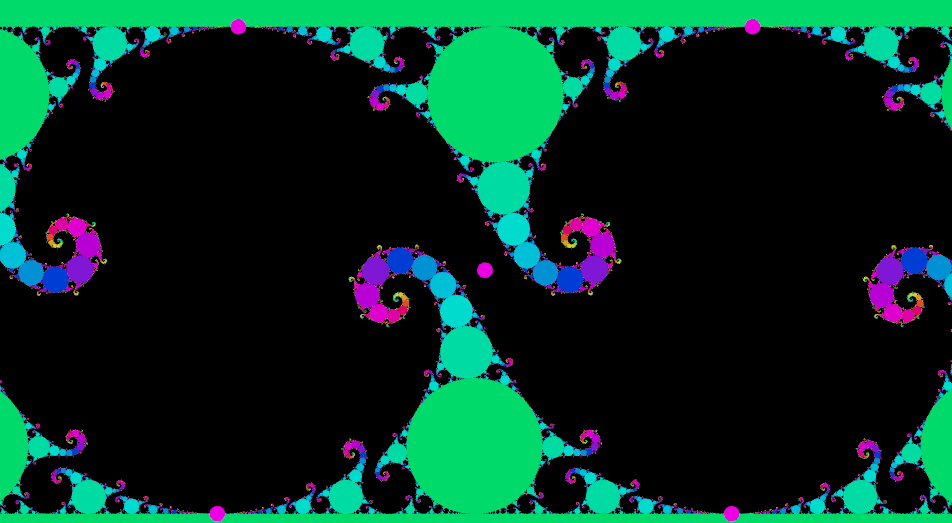
\includegraphics[height=1.35in, keepaspectratio]{img/preparation/related/josklein.png}
  \caption{\textit{}}
  \label{fig:jos}
  \hspace*{\fill}
 \end{minipage}
 \begin{minipage}[t]{0.5\hsize}
  \center
  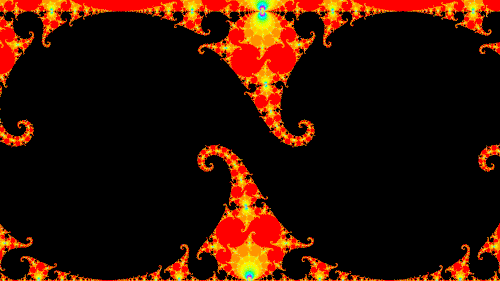
\includegraphics[height=1.35in, keepaspectratio]{img/preparation/related/joskleinInv.png}
  \caption{\textit{}}
  \label{fig:josInv}
  \hspace*{\fill}
 \end{minipage}
\end{figure}

Jos Leys invented efficient algorithm to draw Kleinian group with Maskit
parametrization shown in Figure \ref{fig:jos}\footnote{\url{http://www.josleys.com/article_show.php?id=221}}.
IIS uses circle or sphere inversions on the other hand Jos Leys used
M\"obius transformations algebraically.
He observe the orbit of the maskit parametrization group and 
We can apply circle inversions to his figure, and we obtain Figure \ref{fig:josInv}.

Martin von Gagern and Jürgen Richter-Gebert introduce similar algorithm
called \textit{Reverse Pixel Lookup}
\cite{journals/combinatorics/GagernR09} to render two dimensional hyperbolic tiling.
We explore the method not only tiling but also other varieties of
images for instance, three dimensional objects.
